% use command pdflatex filename.tex
\documentclass{article}
% \usepackage[noend]{algpseudocode}
% \usepackage{parskip}
% \usepackage{tikz, changepage, amssymb}
% \usetikzlibrary{automata,positioning,arrows}
\usepackage{amsmath, amsthm}
\usepackage{listings}
\usepackage{xcolor}
\usepackage{tikz}
\usepackage{array}
\usepackage{url, hyperref}
\usepackage{graphicx, caption}
\graphicspath{{./images/}}


\lstset{
  language=python,
  basicstyle=\ttfamily,
  mathescape,
  morecomment=[l][\color{olive}]{\#},
  breaklines=true,
  postbreak=\space
}
\title{DATASCI 2G03 Project Report \\\large
Elastic Collisions between Contained Particles}
\author{Anthony Hunt}

\begin{document}
\maketitle

\tableofcontents

\section{Introduction}
Visualizing the effects of colliding elastic objects enables a clearer understanding of extremely small or extremely large natural phenomena,
especially in the fields of astrophysics (eg. rotation of stars in a galaxy) and chemistry (eg. ideal gas, electron/proton interactions).
Tools of this nature can provide intuition and a sense of familiarity to those studying these areas.
Even in everyday life, this type of simulation often appears in video games like pong, brick breaker, and 8 ball pool.
Therefore, this project attempts to simulate interactions between a large number of objects through
the motion and collision of moving particles.

The simplest of these interactions are those that do not involve a change in acceleration,
such as an ideal gas in a finite box. Wikipedia has an excellent example of one such simulation
\footnote{\url{https://en.wikipedia.org/wiki/Maxwell\%E2\%80\%93Boltzmann_distribution}}.
% \footnote{\url{https://en.wikipedia.org/wiki/Maxwell\%E2\%80\%93Boltzmann_distribution#/media/File:Simulation_of_gas_for_relaxation_demonstration.gif}}.
Further, a reasonable simulation should expect to converge to the Maxwell-Boltzmann distribution,
a chi-distribution with 3 degrees of freedom \footnote{\url{https://en.wikipedia.org/wiki/Chi_distribution}},
characterized by the large density of particles around the mean and the slow taper for higher particle speeds.

The first part of this project will consist of modelling the interaction between many particles
in a containing box the hopes of achieving a 2D Maxwell-Boltzmann distribution of velocities.
We also ensure correctness of our simulation by monitoring kinetic energy conservation for the system.
Then, we will extend these interactions with the addition of charged particles to simulate the effects of non-constant acceleration.
We do not expect the charged particles to follow the Maxwell-Boltzmann distribution,
but will explore other effects of remote particle-particle interactions, like orbits.


\section{Method}
\subsection{ODE Solver}
Since this simulation is based primarily around dynamic motion,
we will use the kick-drift-kick form of Leap Frog integration
\footnote{\url{https://en.wikipedia.org/wiki/Leapfrog_integration}}:
\begin{align}
    v_{i+\frac{1}{2}}&=v_{i}+a_{i}{\frac {\Delta t}{2}}\\
    x_{i+1}&=x_{i}+v_{i+\frac{1}{2}}\Delta t\\
    v_{i+1}&=v_{i+\frac{1}{2}}+a_{i+1}{\frac {\Delta t}{2}}
\end{align}

\subsection{Initial Equations}

The physics-based ODEs and other equations used to simulate this problem are listed below.
The goal of this simulation is to track the position of objects (represented by $x$)
over some length of time $t$. Each particle will have some mass $m$ and starting velocity $v$.

Velocity ($v$) of one particle
\footnote{\url{https://en.wikipedia.org/wiki/Equations_of_motion}}:
\begin{equation}
    v = \frac{dx}{dt}
\end{equation}

Acceleration ($a$) of one particle:
\begin{equation}
    a = \frac{dv}{dt} = \frac{d^2x}{dt^2}
\end{equation}

Kinetic energy of one particle:
\begin{equation}
E_k = \frac{1}{2}mv^2
\end{equation}

The below equation is used to calculate the vectors of velocity resulting from an elastic collision
\footnote{\url{https://en.wikipedia.org/wiki/Elastic_collision}}.
Let $v_1$ represent the first particle's velocity and $v_2$ for the second particle's velocity.
Additionally, let $v'$ represent the velocity after the collision and $v$ for the velocities prior to the collision.
Swapping $*_1$ and $*_2$ will provide the velocity for particle 2.

\begin{equation}
v'_1 = v_1 - \frac{2m_2}{m_1+m_2}\frac{\langle v_1 - v_2, x_1 - x_2 \rangle}{\|x_1-x_2\|^2}(x_1-x_2)
\end{equation}

\subsection{Extended Equations}

Newton's second law:
\begin{equation}
F = ma
\end{equation}

Coulomb's law: Force of charged particles against one another:
\begin{equation}
    F_{charge} = \frac{kq_1q_2}{r^2}
\end{equation}

Electric potential energy of a system
\footnote{\url{https://phys.libretexts.org/Bookshelves/University_Physics/University_Physics_(OpenStax)/University_Physics_II_-_Thermodynamics_Electricity_and_Magnetism_(OpenStax)/07\%3A_Electric_Potential/7.02\%3A_Electric_Potential_Energy}}:

\begin{equation}
    U = \frac{k}{2} \sum_i^N \sum_j^N \frac{q_iq_j}{r_{ij}} \text{for} i \neq j
\end{equation}

\subsection{Configuration Parameters}
\begin{itemize}
    \item Starting position $s$ of each particle
    \item Initial velocity $v$ of each particle
    \item Mass $m$ of each particle (kept at a constant 1 kg except for configuration 9)
    \item Radius of each particle $r$ (kept at a constant 0.25 m)
    \item Charge of different particles $q$ (kept at a constant $\pm 1$ except for configuration 9)
    \item Coulomb's constant $k$ (kept at $5 Nm^2/C$ instead of $9\times 10^9 Nm^2/C$ since we are massively downscaling real-world values)
\end{itemize}

\subsection{Interesting Properties}
\begin{itemize}
    \item Speed of particles over time (momentum of all particles should remain constant) position of particles on a graph
    \item Distribution of particle speeds (Maxwell-Boltzmann distribution)
    \item Unique path of each particle (random movement of one particle) \footnote{\url{https://en.wikipedia.org/wiki/Brownian_motion}}
\end{itemize}

\section{Testing}
To ensure the correctness of our program,
we compare the results of a few preset configurations against the expected behaviour of the simulation.
Additionally, we examine a collection of randomly positioned particles.

\subsection{Uncharged Particles}
The tests for this section cover the initial model of this project, without any extensions.
All particles are set to a charge of 0, so they only interact though collisions with other particles and walls.
This setup mimics that of an ideal gas, so we are expecting to find that energy is conserved and
the distribution of speed eventually forms the Maxwell-Boltzmann curve.

\subsubsection{2 Particles in a 1D Collision}
This test examines the effects of one collision between two particles moving towards one another on the x-axis,
as shown below. Both particles have the same initial speed and are pointed towards the origin:
\\
\begin{center}
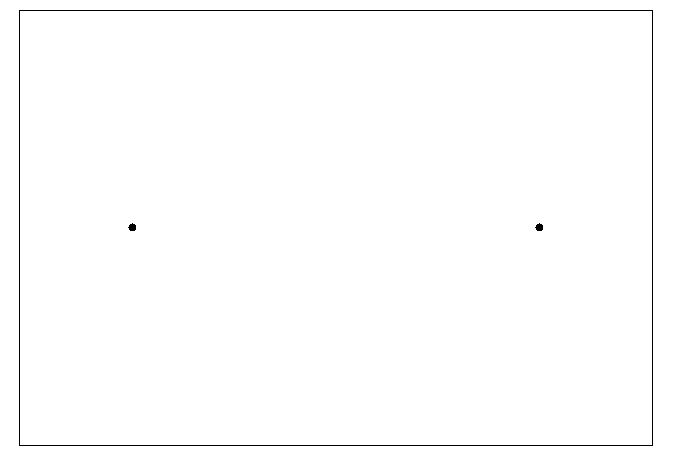
\includegraphics[scale=0.5]{uncharged_2_particles_1D}
\captionof{figure}{Two uncharged particles aligned on the x-axis. Initial velocities are equal and towards the origin.}
\end{center}

Plotting the total energy and speed over time (blue and green respectively),
we find that kinetic energy is entirely conserved.
The purple line indicates electric potential energy and can be ignored for now.
Note that there is no scale for the Time axis since this graph updates by appending new data every $dt$ seconds.
This means that initial iterations take up the entire plot and then compress as time goes on
and the plot holds more data.
\\
\begin{center}
    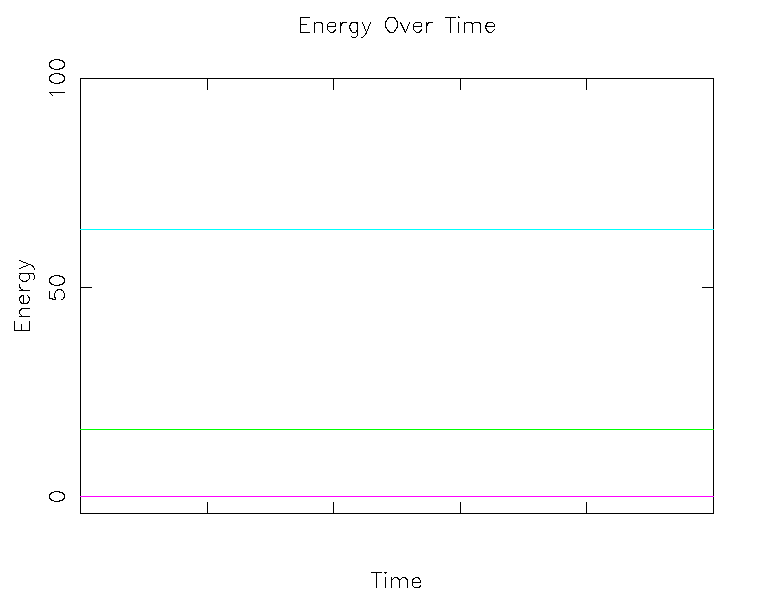
\includegraphics[scale=0.5]{uncharged_2_particles_1D_energy}
\captionof{figure}{Energy over time for the collision of two particles. Kinetic energy (blue), speed (green), electric potential energy (pink), and total energy (black, obscured by and equal to kinetic energy) are constant.}
\end{center}

\subsubsection{2 Particles in an Angled Collision}
Similar to the previous test, but we now check that the angle of deflection for both particles are correct.
A simple case for examining angles is to move the point previously located at $(-1,0)$ to $(0,1)$ and point it towards the origin.
Thus, the two particles will meet at a 90-degree angle and bounce in perpendicular directions.
The initial layout of this test has particles located at the top and right with velocities toward the origin:
\\
\begin{center}
    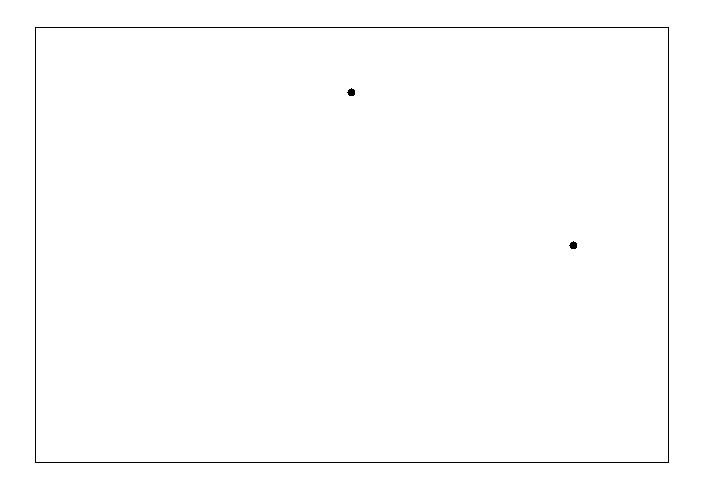
\includegraphics[scale=0.5]{uncharged_2_2D_start}
    \captionof{figure}{Particles at the top and right, facing towards the origin.}
\end{center}

After collision, the initially top particle will be sent to the left and the right particle to the bottom.
Since the particles met at a 90-degree angle, they must depart at 90-degrees in order to conserve momentum
towards the bottom left.
\\
\begin{center}
    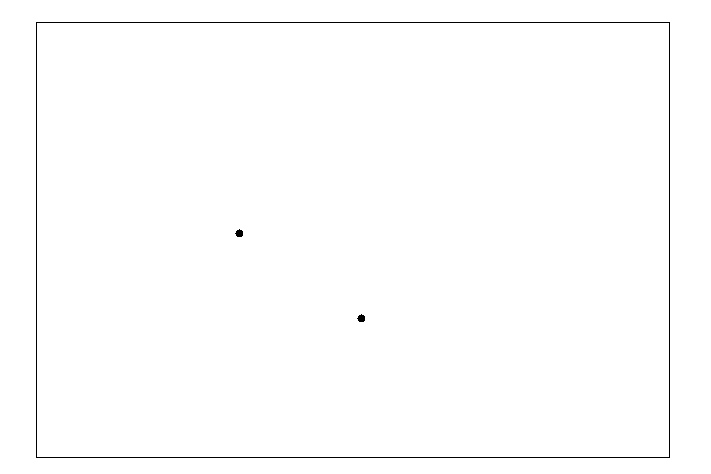
\includegraphics[scale=0.5]{uncharged_2_2D_after}
    \captionof{figure}{Particles at the bottom and left, after a 90-degree collision at the origin.}
\end{center}

The particles will then bounce against the walls, reversing direction and colliding at the origin again.
Particle locations will swap between the two quadrants until the simulation is stopped.
Energy is conserved during this as both particles bounce with the same net speed
(although we do not include the energy vs time graph here since it looks the same as section 3.1.1).

\subsubsection{200 Random Particles}
With a large amount of particles, we can now examine the distribution of speed compared to the Maxwell-Boltzmann distribution.
The speed distribution of particles is separated into 30 ``buckets'',
where each particle is sorted into a bucket based on its speed.
Each bucket holds a range of $1m/s$, where he maximum speed bucket is $30 m/s$
Note that the specific x-axis speeds are not especially important
since it is more important to visualize the groupings of particles rather than the exact speed of the particles themselves.
For example, we could scale down the interpreted particle speeds based on the maximum speed and receive a similar graph.

An image of the simulated particles is below:
\\
\begin{center}
    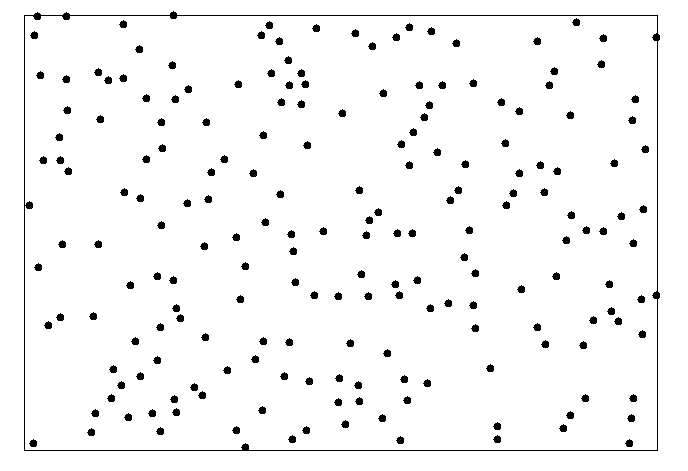
\includegraphics[scale=0.5]{uncharged_random}
    \captionof{figure}{200 particles with initially random positions and velocities.}
\end{center}

After a few seconds of simulation, the distribution graph for 200 particles visibly relaxes from a random distribution
into the Maxwell-Boltzmann distribution.
\\
\begin{center}
    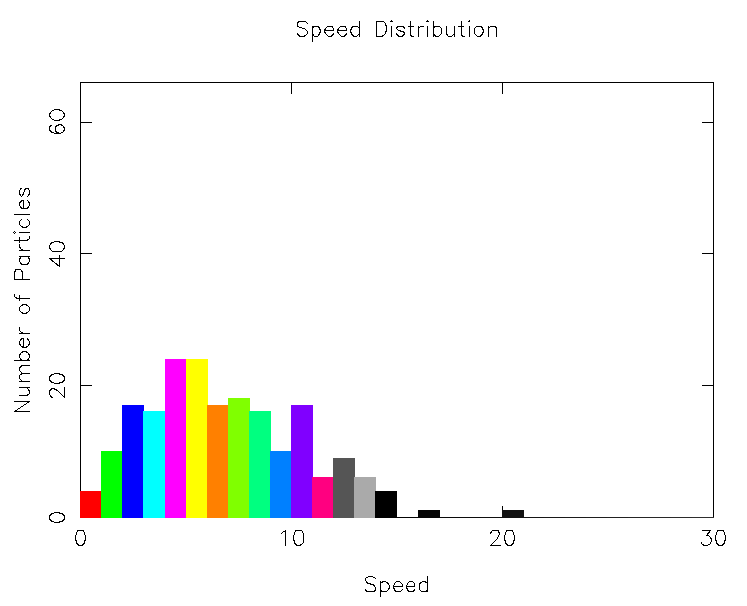
\includegraphics[scale=0.5]{uncharged_random_dist}
    \captionof{figure}{Speed distribution of 200 random particles. Most particles stay within the 2 to $12 m/s$ range}
\end{center}

Calculating the exact curve of the distribution is slightly out of the scope of this project
since we do not collect any information on gas-specific statistics (ie., temperature, pressure, heat),
but the characteristic bulge and slow taper can be visually estimated and compared with Wikipedia's simulation:
\\
\begin{center}
    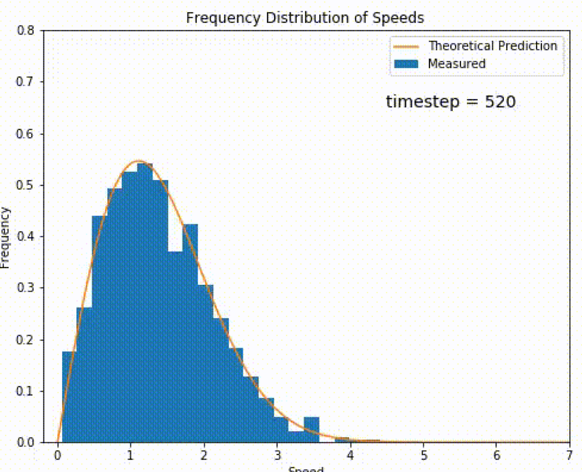
\includegraphics[scale=0.5]{mb_wiki}
    \captionof{figure}{Wikipedia image of the Maxwell-Boltzman distribution against the actual speed distribution of particles.}
\end{center}

Finally, we see that kinetic energy is indeed conserved, although total speed fluctuates within a margin of error.
\\
\begin{center}
    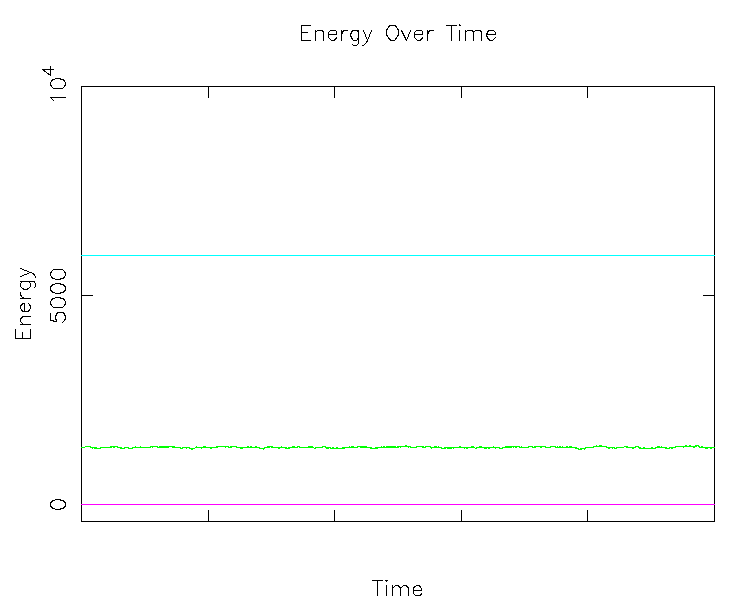
\includegraphics[scale=0.5]{uncharged_random_energy}
\captionof{figure}{Energy over time for the collision of 200 particles. Kinetic energy (blue), speed (green), electric potential energy (pink), and total energy (black, obscured by and equal to kinetic energy) are constant.}
\end{center}

\subsection{Charged Particles}
The inclusion of charged particles within the simulation adds an additional ODE for our consideration,
namely, a non-constant acceleration due to Coulomb's Law.
The focus of this extension is to demonstrate how equations for dynamic particle movement
can be manipulated and reused to provide an idea of orbital movement.
Similar to gravity, the acceleration of charged particles is remotely influenced through other nearby particles.

\subsubsection{2 Particles Interacting in 1D}
The same experiment for uncharged particles can be performed on charged particles.

For particles with the same charge, the setup is as follows (initial velocity towards the origin):
\\
\begin{center}
    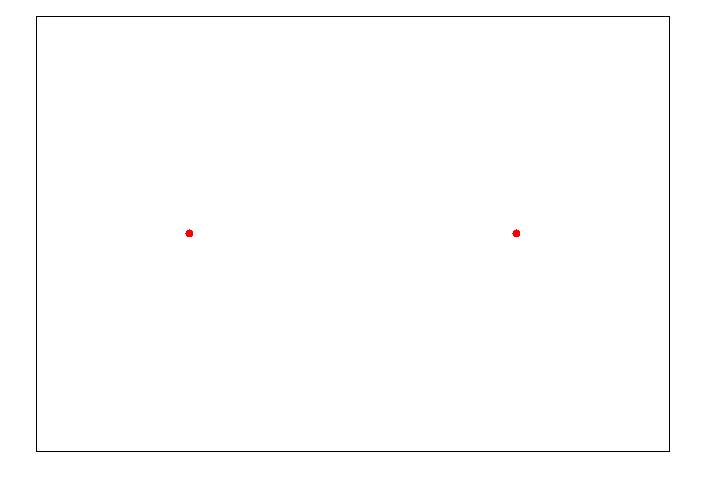
\includegraphics[scale=0.5]{charged_2_same}
    \captionof{figure}{Two positively charged particles with initial velocities towards the origin.}
\end{center}

As the particles approach one another, their speed and kinetic energy transform into electric potential energy.
Eventually, the particles stop a small distance before collisions and begin moving in the opposite direction.
Then, when moving apart, the potential energy is converted back into kinetic and the particles speed into the wall.
An oscillation pattern between the kinetic energy (blue) and electric potential (pink) can be seen below.
Note that the total energy of the system (black) is conserved throughout and total speed (green) follows the kinetic energy.
\\
\begin{center}
    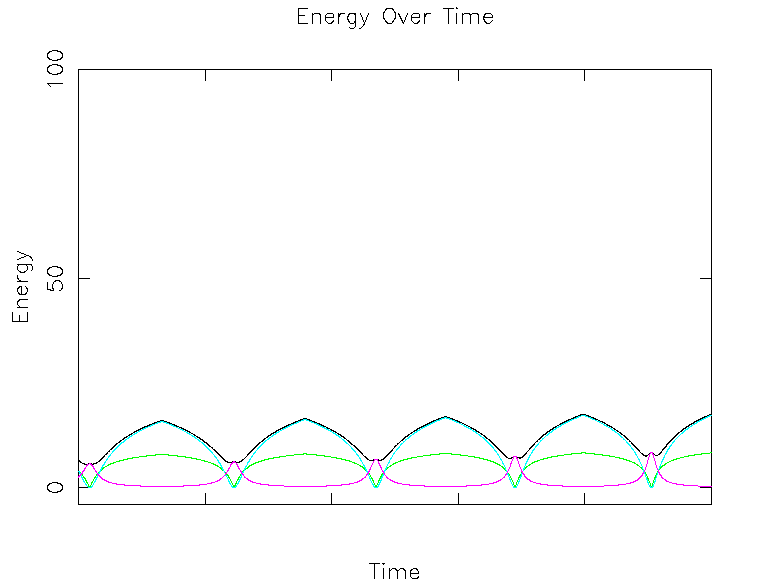
\includegraphics[scale=0.5]{charged_2_same_energy}
    \captionof{figure}{Energy over time for two positively charged particles. Note that electric (pink) and kinetic (blue) energy oscillate but always add up to the total energy (black).}
\end{center}

Similar behaviour can be seen for opposite charges, with the energy curves flipped.
There is a slight, repeated fluctuation in total energy at the moment of collision,
but the overall energy of the system does not change.
\\
\begin{center}
    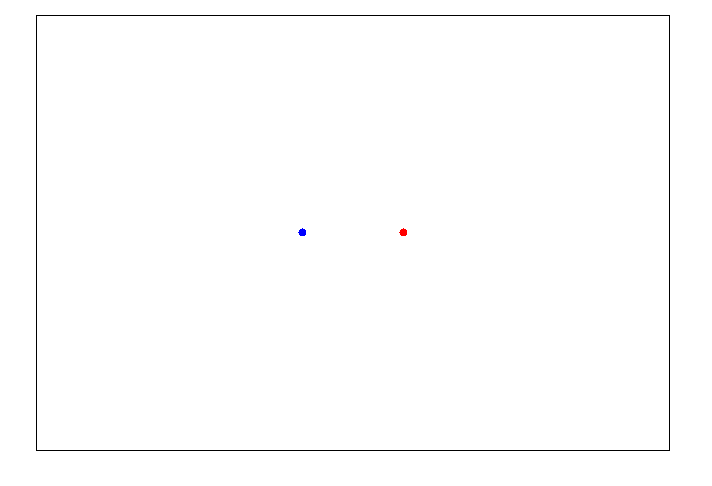
\includegraphics[scale=0.5]{charged_2_opp}
    \captionof{figure}{Two oppositely charged particles with initial velocities towards the origin.}
    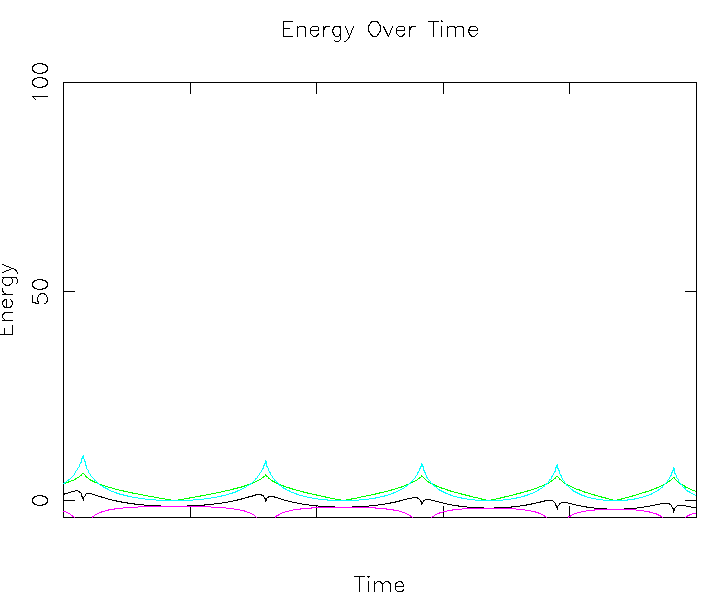
\includegraphics[scale=0.5]{charged_2_opp_energy}
    \captionof{figure}{Energy over time for two oppositely charged particles. Once again, electric (pink) and kinetic (blue) energy oscillate but always add up to the total energy (black).}
\end{center}



\subsubsection{Orbiting Particles}
The below setup places two oppositely charged particles at equal and opposite distances from the origin, with initial velocity parallel to the y-axis.
This led to a stable elliptical orbit about the origin.
\\
\begin{center}
    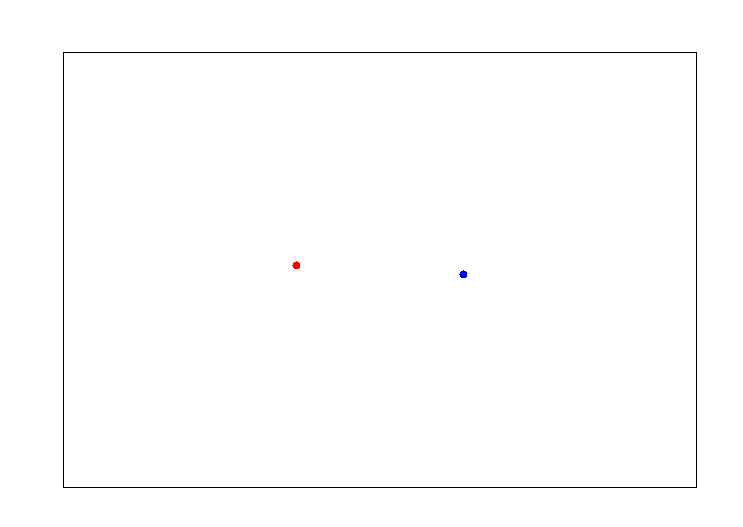
\includegraphics[scale=0.5]{orbit}
    \captionof{figure}{Two particles orbiting about the origin. The blue particle has velocity downward, while the red particle has velocity upward.}
\end{center}

In the below graph, fluctuations in kinetic energy (blue) and electric potential energy (pink) oscillate opposite to one another,
as the two particles get closer/faster and further/slower to one another.
We still note that the total energy (black) remains constant throughout.
\\
\begin{center}
    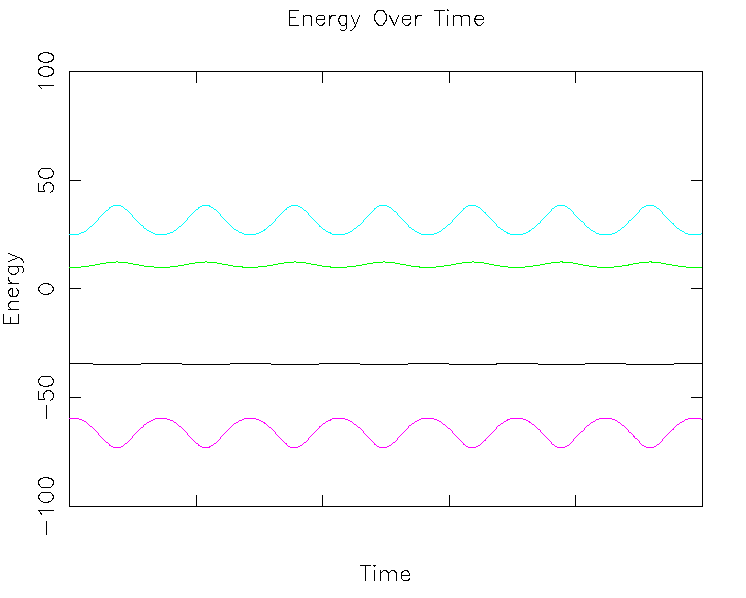
\includegraphics[scale=0.5]{orbit_energy}
    \captionof{figure}{Energy over time between orbiting particles. Electric (pink) and kinetic (blue) energy oscillate and sum to total (black). }
\end{center}

Orbits akin to Bohr-Rutherford models of the atom,
where small charges orbit a large central charge,
can be seen by configuring several negatively charged masses initially travelling
perpendicular to the electric force from a large red mass.
The energy over time is shown below, following the same oscillation as above.
\\
\begin{center}
    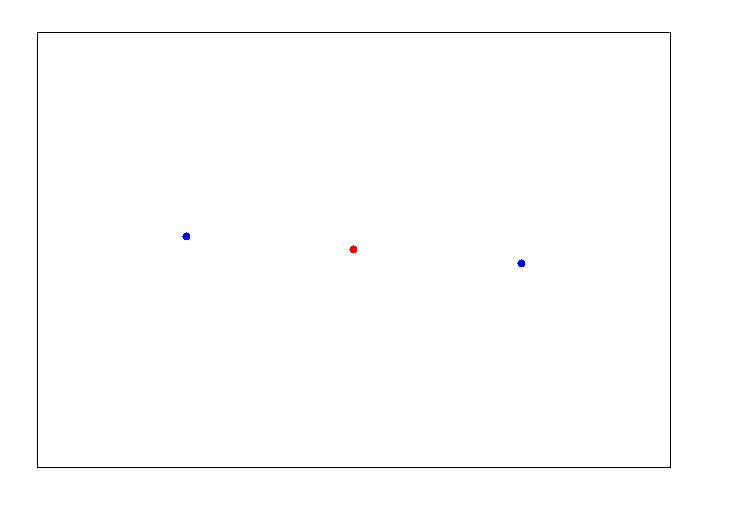
\includegraphics[scale=0.5]{atom}
    \captionof{figure}{Two negatively charged low-mass particles orbiting a highly positively charged central particle, akin to electrons and protons in an atom.}
    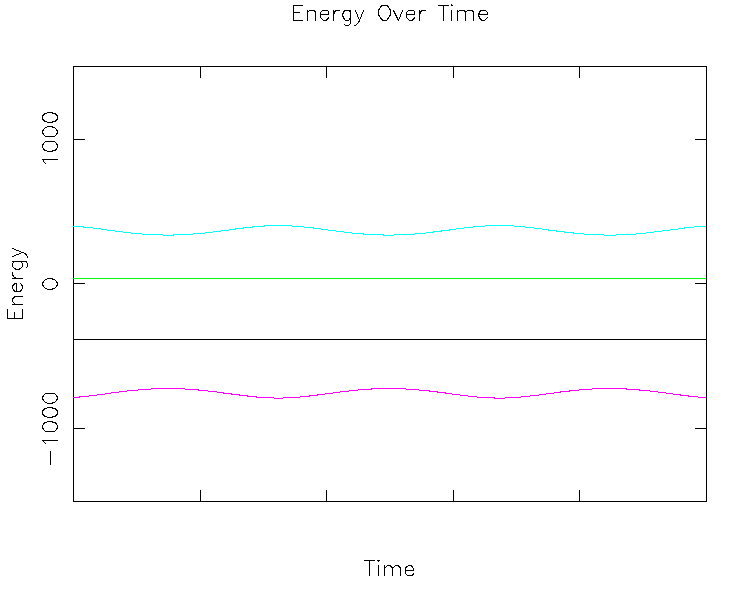
\includegraphics[scale=0.5]{atom_energy}
    \captionof{figure}{Energy over time for particles orbiting around another particle. Electric (pink) and kinetic (blue) energy oscillate and sum to total (black). }
\end{center}

\subsubsection{200 Random Particles}
This test is similar to that of the uncharged particles,
but all particles have been either assigned a positive (red) or negative (blue) charge.
The setup and energy graphs are listed below:
\\
\begin{center}
    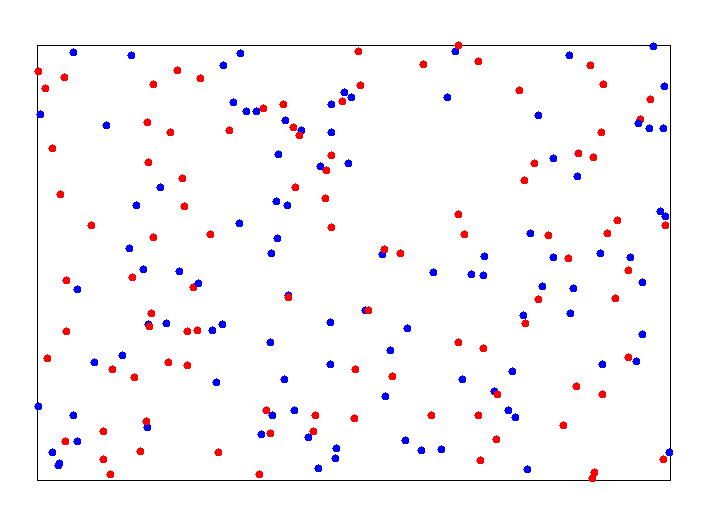
\includegraphics[scale=0.5]{charged_random}
    \captionof{figure}{200 randomly charged particles.}
    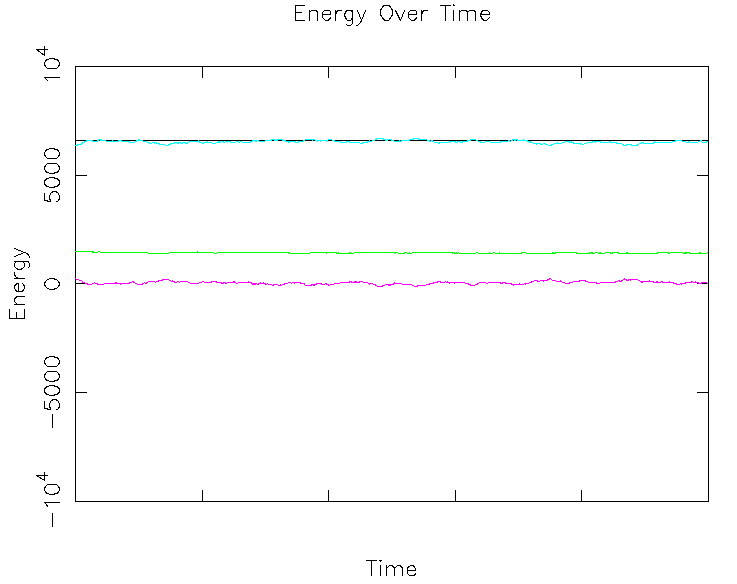
\includegraphics[scale=0.5]{charged_random_energy}
    \captionof{figure}{Energy over time for 200 randomly charged particles. The total energy (black) remains constant.}
\end{center}

These random particles have a similar shape to the Maxwell-Boltzmann distribution,
likely due to the high ratio of kinetic to electric potential energy.
\\
\begin{center}
    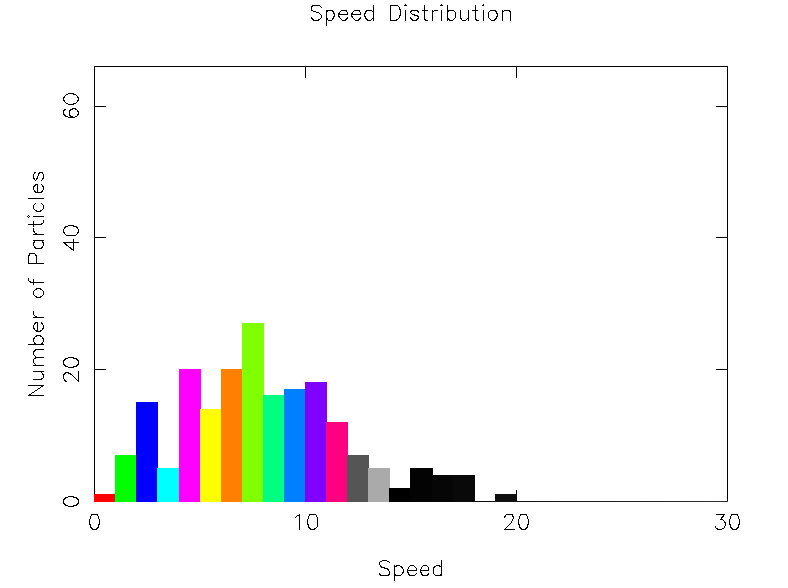
\includegraphics[scale=0.5]{charged_random_dist}
    \captionof{figure}{Speed distribution 200 randomly charged particles, appearing similar to the Maxwell-Boltzman distribution.}
\end{center}


\section{Results}
% The nature of this project and my simulation model is such that most interesting visuals
% are the result of viewing updating graphs in real time.
% Since snapshots of the model have been included as part of initial configuration for several tests above,
% this section does not include any additional figures.
% For consistency, this section only contains an analysis of the initial and extended tests described in section 3.
Overall, both models of uncharged and charged particles behaved as expected
with respect to energy conservation and speed distribution.
Selected tests also demonstrated the conservation of momentum and distance-based forces.
Outside of exceptional circumstances, Leap Frog integration had a high degree of precision throughout all iterations of the simulation,
demonstrating its effectiveness for dynamic systems.

\subsection{Initial Model - Uncharged Particles}
Initially, I faced difficulties with conservation of kinetic energy for uncharged particles
since some collisions would last for longer than one $dt$ instant.
To counter this, I implemented a directional check to ensure that particles only
collide when they are facing towards one another
\footnote{Dr. Wadsley initially told me about the equation, but the linked forum post also states the same method:
\url{https://math.stackexchange.com/questions/1438002/determine-if-objects-are-moving-towards-each-other}}.

Along with the above bug in collision calculations, I had also mistakenly tried calculating new velocities
based on the contributions of each particle at one point in time.
However, doing so led to very unpredictable behaviour when 3 or more particles collided at once, where
involved particles would either explode with speed or slow down immensely.
Eventually, this was resolved by calculating the pairwise collisions of every particle in some arbitrarily chosen order.

Although the energy-time graphs are not very interesting in section 3.1,
they serve as a constant, visual examination of the total energy of the system.
For a simulation with no explicit acceleration changes, all lines on the graph should and do appear as flat line.

\subsubsection{Extended Testing: 8-Ball Pool with 225 Particles}
From the experiment in section 3.1.3, we can hypothesize that given a high enough density of particles in an enclosed space,
the initial distribution does not matter. To test this claim, we select an experiment grounded with the real world:
what would happen if we removed the friction and pockets from a pool table when making a ``break'' shot?
For better visualization of the Maxwell-Boltzman distribution, we increase the number of balls on the pool table to 200.
The initial layout of the test is shown in the following figure along with the initial speed distribution.
Note that only one particle is moving to the right at $100 m/s$ while all others are at rest.
\\
\begin{center}
    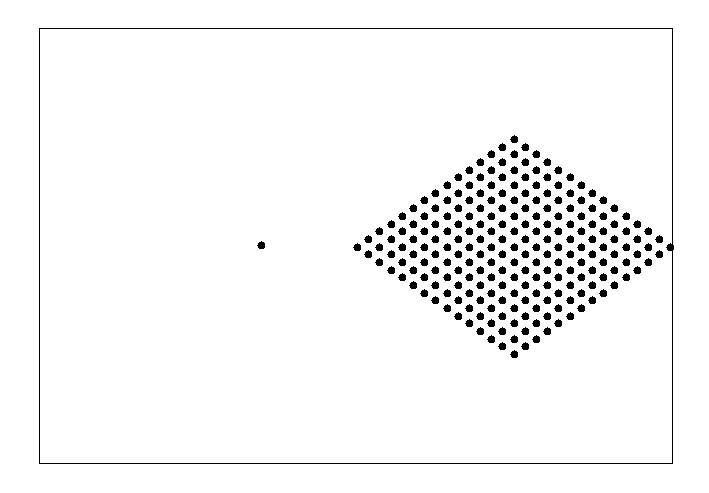
\includegraphics[scale=0.5]{uncharged_pool}
    \captionof{figure}{Initial setup similar to the game of 8-ball pool. One high-speed particle from the left strikes a diamond of still particles.}
    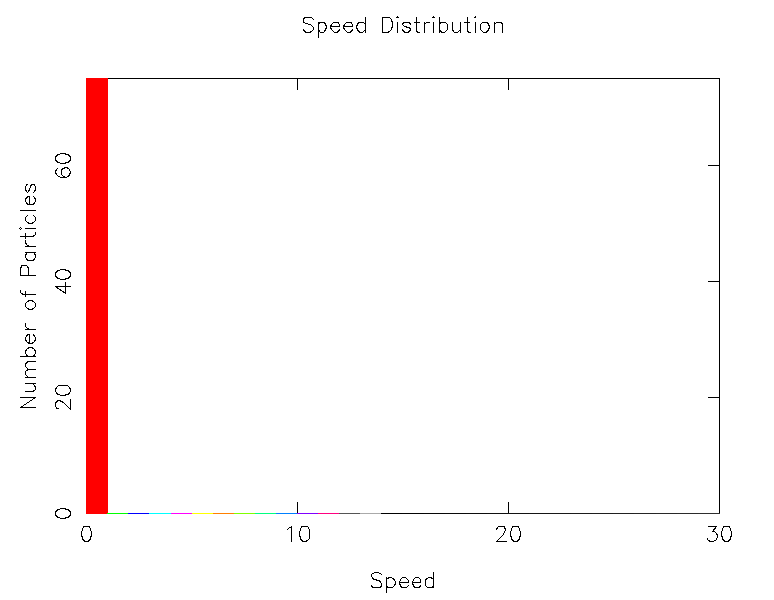
\includegraphics[scale=0.5]{uncharged_pool_dist}
    \captionof{figure}{Initial speed distribution for the above setup. All particles are at rest, except for the ``cue'' ball, which has a speed $>30m/s$.}
\end{center}

After about one minute, we see a very similar result as in section 3.1.3. In fact, aside from the differences in initial energy,
the two plots are nearly indistinguishable.
\\
\begin{center}
    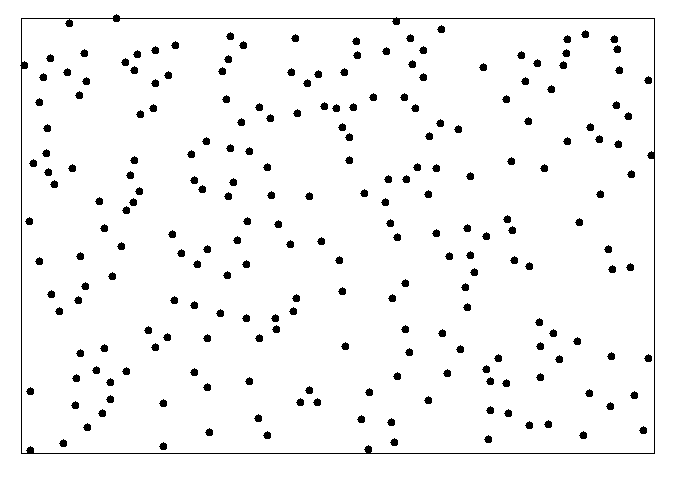
\includegraphics[scale=0.5]{uncharged_pool_2}
    \captionof{figure}{Particles of the pool setup after some time. The random movement is similar to that of the 200 random particles}
    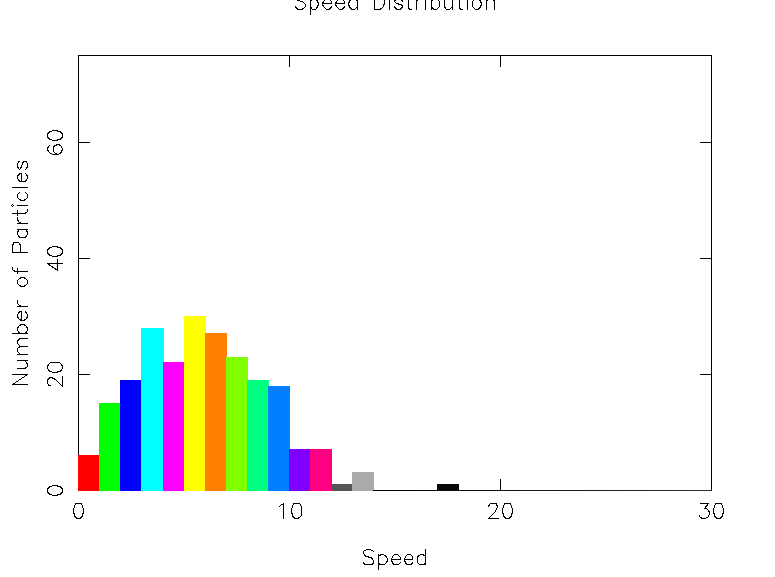
\includegraphics[scale=0.5]{uncharged_pool_dist_2}
    \captionof{figure}{Speed distribution the pool setup after some time. The shape of the curve is similar to that of the 200 random particles}
\end{center}

\subsection{Extended Model - Charged Particles}
Since charged particles were used with a mass of $1 kg$ and charges equal to $\pm 1 C$,
a far lower Coulomb constant $k$ was necessary to prevent extreme changes in acceleration.
Dealing with extreme values in the case of charged particles was especially difficult,
as small errors in transforming continuous phenomena into discrete often occurred as a result of
particles escaping the boundaries or coming in close contact with one another.

Enabling collisions during testing produced all results as expected
with respect to the conservation of energy and distribution of speed
In the case of two charged particles interacting with one another,
the oscillation between kinetic and electric potential energy matched
expectations and maintained conservation rules.

For tests with collisions disabled, as mentioned in section 3.2.1,
monotonic changes in the total system energy could be caused
by a combination of the transition to discrete steps and
the soft max function limiting acceleration due to surrounding charges.

While the charged particle model massively simplifies all the complex interactions between particles in the real world,
the visualization of interacting particles is more than reasonable for most common configurations.
With the charged model, we can plainly see physical phenomena like orbital movement as a product of a constant central acceleration
and an appropriate starting velocity.

\subsubsection{Extended Testing: 2 Particles Interacting in 1D Without Collisions}
This section is an extension of section 3.2.1.

For particles of opposite charge, the total energy of the system remained constant when collisions were enabled.
However, when collisions were disabled (so that particles had a radius of 0 and could become arbitrarily close to one another),
the energy of the system behaved erratically.
Disabled collisions allowed
the particles to pass through one another (and the distance between them to become infinitesimally small) rather than colliding.
This drastic change in behaviour is likely due to the imprecision of integration at high acceleration and velocity values.
Consider the following timeline for two particles:
\begin{itemize}
    \item The two particles start far away and move towards one another at a moderate but increasing velocity
    \item At some critical point, the particles reach their closest point. They experience a high force of attraction
    \item The first part of Leap Frog converts that high acceleration into high velocity, enough such that the particles swap places.
    In other words, the particle on the right is now on the left and vice versa.
    \item Leap Frog then recalculates the force of acceleration, based on the new particle positions.
    However, the two particles are farther apart from one another than they were in step 2.
    Thus, the new force of acceleration is opposite but not equal to that step.
    \item Since there is asymmetry in the moments before and after the particles swapped places,
    the particles zoom into the bounding walls before meeting again and performing the reverse.
\end{itemize}
% In particular, if two particles are extremely close at one point in time but
% accelerate very far in the opposite direction the next moment, the increased
% kinetic energy from the first moment does not get a chance to convert back to electric potential energy after the particles have swapped positions.
We have attempted to mitigate these errors through an additional epsilon term to prevent the distance of two particles from reaching 0,
but the above situation is still applicable.
All previous tests, have collisions enabled to remove errors of this kind.
The second graph below is the same as the first energy-time graph with $dt$ set to half of the original time step.
The final graph is the energy over time at a tenth of the original time step.
\\
\begin{center}
    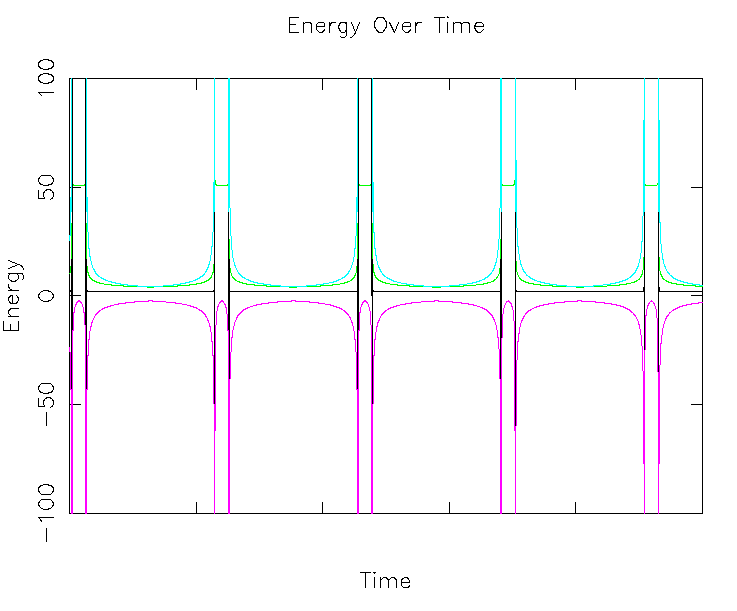
\includegraphics[scale=0.5]{charged_2_opp_energy_no_collision}
    \captionof{figure}{Energy over time for two oppositely charged particles with no radius (collisions disabled).}
    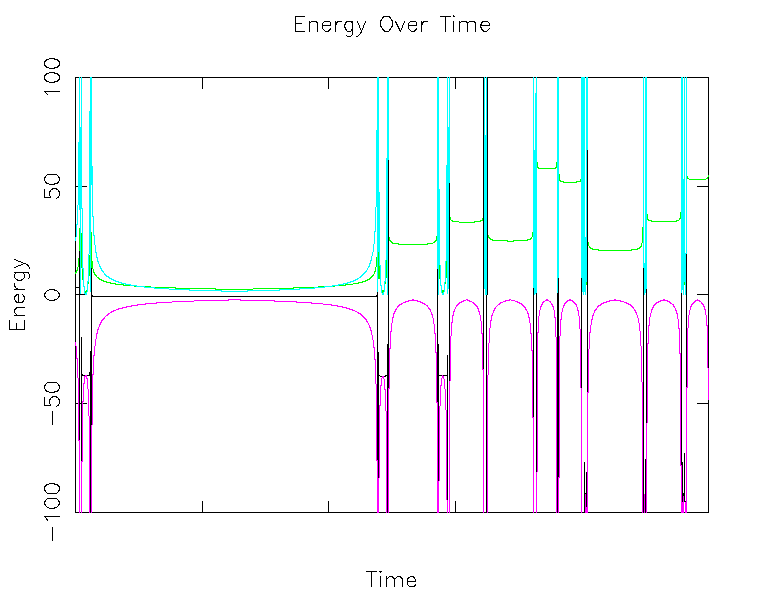
\includegraphics[scale=0.5]{charged_2_opp_energy_no_collision_half_time}
    \captionof{figure}{Same as above, but with $dt = 0.005s$ (half of above)}
    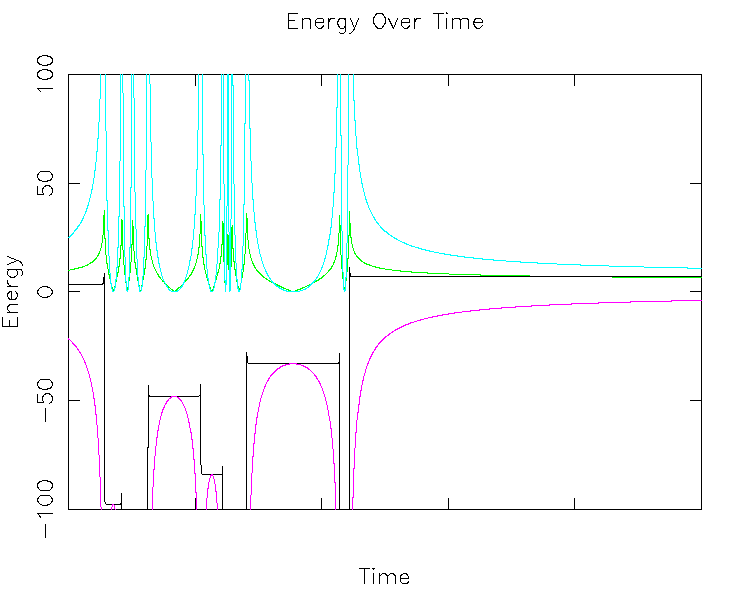
\includegraphics[scale=0.5]{charged_2_opp_energy_no_collision_tenth_time}
    \captionof{figure}{Same as above, but with $dt = 0.001s$ (a tenth of the first graph)}
\end{center}


\section{Conclusion}
Both models performed well to simulate moving particles,
but there is far more that could be done to explore this topic further:
\begin{itemize}
    \item Incorporation of gravity as an optional force.
    Implementing this with the current state of my project should not be terribly difficult,
    since a developer would only need to add the force of gravity to the collection of acceleration contributions.
    The two independent variables required to calculate gravitational force (mass and distance) are readily accessible within each particle's object.
    \item Expanding the container to a variety of different shapes.
    This would necessarily involve improvements to wall collision calculations in accommodating angles or curves.
    \item Improve wall bounce calculations to ensure that out-of-bounds objects are pushed back in bounds.
    Currently, if objects have enough velocity and acceleration away from the origin, the naive velocity reversal
    calculations of \texttt{Container::get\_collision\_velocity} may not be enough to keep it in bounds.
    \item Improve program efficiency from $O(n^2)$ to $O(n\log{n})$ by dividing the space
    and calculating collisions only for those objects close to one another.
    One of the more recent lectures have also explored an optimal
    method of calculating distant-dependent forces using a divide and conquer method.
    \item Add friction or an electric field map to provide non-constant acceleration outside of particle-particle interactions.
    This would enable the model to run other physics-based simulations like a mass spectrometer or even projectile motion
    (eg. a positively charged particle moving parallel to a negatively charged bottom plate).
    \item Count the number of collisions between particles against a wall.
    3Blue1Brown has an excellent video exploring a special case where large
    masses collide with small masses with a ratio $\pi\times 10^x$ where $x$ is based on the ratio of the object masses
    \footnote{\url{https://www.youtube.com/watch?v=jsYwFizhncE}}.
    \item Examine the overall (conservation of) momentum of the system over time.
    The visualization of momentum could be plotted on the moving particle graph with vectors showing the momentum of each particle.
    \item Calculations for pressure, temperature, etc. in the context of the ideal gas law.
    This would also enable a direct overlay of the Maxwell-Boltzman distribution on the energy distribution graphs seen above.
    \item Interactivity improvements, like adding energy to the system in the form of heat, controlling select particles,
    or tracing the path of selected particles to find random walk behaviour
    \footnote{\url{https://en.wikipedia.org/wiki/Brownian_motion}}.
    Adding containers that react to pressure differences may serve as a more realistic simulation of the physical world.
\end{itemize}

Exploring and researching about particle simulation in the context of C++
helped me gain a deeper understanding and appreciation of physical interactions.
Among the most interesting findings was the mimicking of orbiting
objects through charged particles with select initial velocities,
the Maxwell-Boltzmann distribution of neutral particles,
and the behaviour of charged particles given pre-selected configurations.
Both models serve as an excellent tool to better visualize and interpret miniscule molecule-level movements.




\end{document}
